\label{chap:back-end}

En aquest capítol es fa referència a la implementació del \emph{back-end} de la aplicació.
Està implementat amb la framework de \texttt{Laravel} \autocite{laravel}
és una framework del llenguatge de programació PHP. S'utilitza per al desenvolupament d'aplicacions web.

\section{Elecció de l'entorn}

En aquesta secció s'explica els punts forts de la eina triada per realitzar el \emph{back-end} de l'aplicació.

\begin{itemize}
    \item És una de les frameworks més utilitzades \autocite{estadistiques_backend}.
    \item L' \texttt{ecosistema}, és a dir la comunitat que hi ha fent-ne ús cada dia.
    Facilita a l'hora de trobar solucions a problemes que es poden trobar al llarg del
    desenvolupament d'una aplicació. També ajuda al fet que sigui una eina on sempre hi
    hagi un manteniment i estigui actualitzada a noves eines per facilitar la feina o fins
    i tot a estalviar-ne.
    \item Laravel inclou \texttt{Eloquent}, mapatge d'objectes relacional (ORM) que fa que sigui
    agradable interactuar amb la base de dades. Cada taula de base de dades té un "Model"
    corresponent que s'utilitza per interactuar amb aquesta taula. A més de recuperar registres
    de la taula de la base de dades, també permeten inserir, actualitzar i eliminar registres
    de la taula \autocite{eloquent_laravel}.
    \item \texttt{Recursos API}, Quan l'aplicació crea una API, és possible que necessiti una capa
    de transformació que es trobi entre els models Eloquent i les respostes JSON que realment
    es retornen als usuaris de l'aplicació. Permet transformar de manera expressiva i senzilla
    els models i co\l.leccions de models en JSON.
    Ofereixen un control més sòlid sobre la serialització JSON dels models i les seves relacions
    \autocite{resources_laravel}.
    \item Una altra eina són les \texttt{migracions}, permet definir i compartir l'esquema de la
    base de dades de l'aplicació \autocite{migrations_laravel}.
    \item L'\texttt{Autenticació}, Laravel s'esforça per oferir les eines necessàries per implementar
    l'autenticació de manera ràpida, segura i senzilla \autocite{auth_laravel}.
    \item Sistema de \texttt{caché} fa que l'aplicació vagi igual de ràpid en local que en producció.
    \item La \texttt{validació de dades}: Laravel ofereix diversos enfocaments diferents per validar
    les dades entrants de l'aplicació, les so\l.licituds HTTP entrants. Inclou una gran varietat de
    regles de validació \autocite{validacio_dades_laravel}.
    \item \texttt{Laravel cashier Stripe} ofereix una interfície expressiva i fluida als serveis de
    facturació de subscripcions de Stripe. Gestiona gairebé tot el codi de facturació de subscripció general i
    d'altres \autocite{cashier_laravel}.
    \item \texttt{Laravel Sanctum} ofereix un sistema d'autenticació lleuger per a SPA
    (aplicacions d'una sola pàgina), aplicacions mòbils i API simples basades en tokens \autocite{sanctum_laravel}.
\end{itemize}

\section{Base de dades}
\label{chap:base_dades}

Qualsevol aplicació interactua amb una base de dades per tal de recopilar i emmagatzemar dades
amb una tècnica ordenada i seguint una estructura coherent i accessible.
Com s'ha esmentat en la secció anterior, Laravel utilitza l'ORM Eloquent.

L'estructura de la base de dades és de la següent manera:

\begin{figure}[H]
\begin{center}
    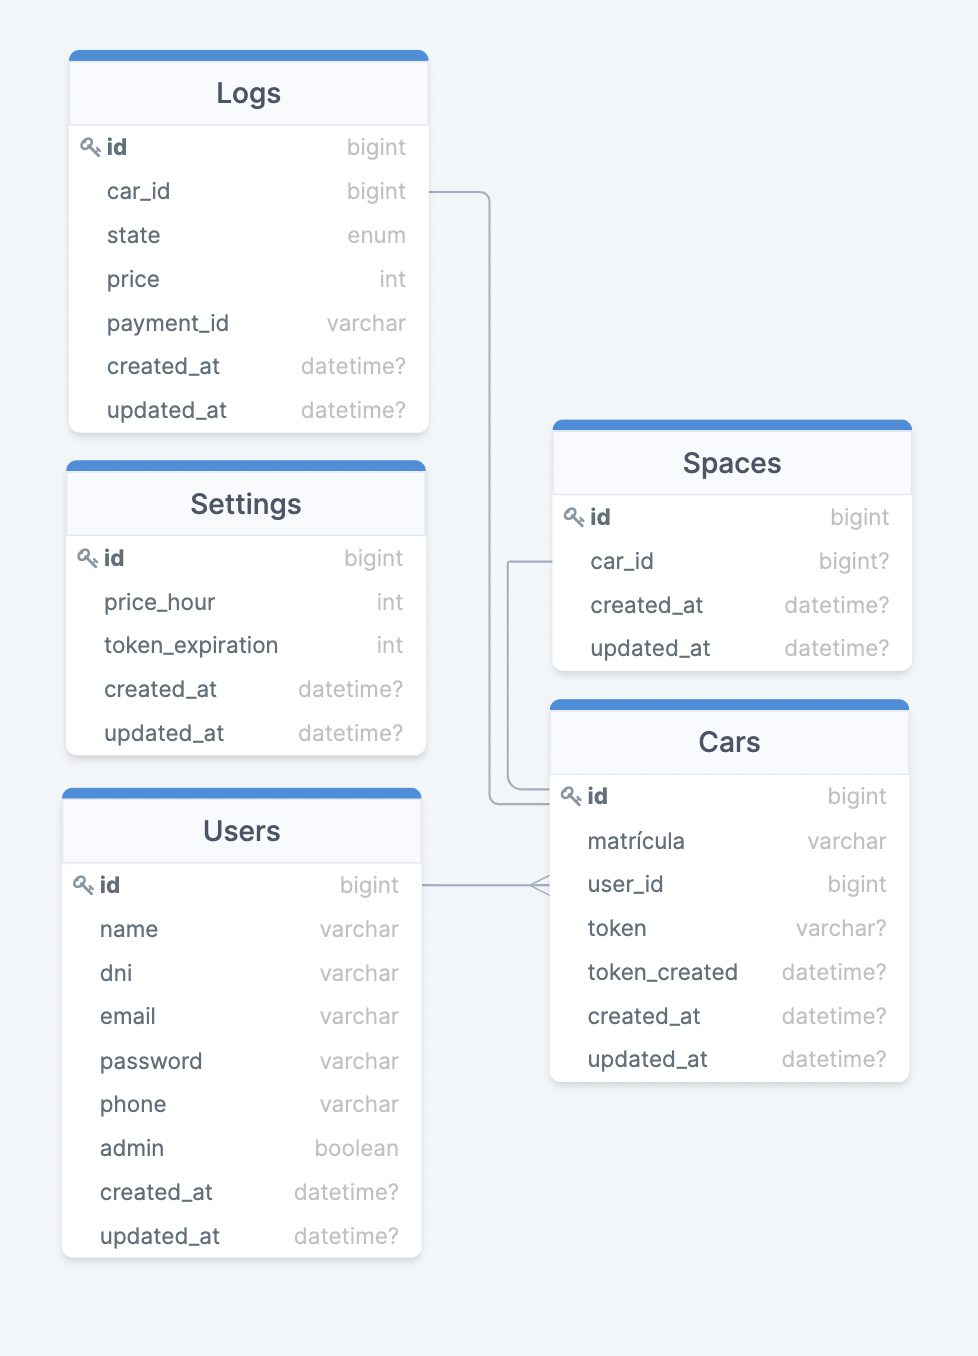
\includegraphics[scale=0.45]{Fotos/BD.png}
\end{center}
\caption{Estructura base de dades}
% \label{fig:BD}
\end{figure}

\begin{table}[H]
\centering
\begin{tabular}{lll}
\hline
\textbf{Columna} & \textbf{Tipus} & \textbf{Descripció}                                                                                             \\ \hline
id               & integer        & \begin{tabular}[c]{@{}l@{}}Clau primària, única per a cada usuari. \\ Autoincrementa el seu valor\end{tabular} \\ \hline
name              & varchar(255)   & Nom i cognom de l'usuari.                                                                                       \\ \hline
dni              & varchar(9)     & \begin{tabular}[c]{@{}l@{}}Número del DNI de cada usuari. \\ Únic per a cada usuari.\end{tabular}               \\ \hline
email            & varchar(255)   & \begin{tabular}[c]{@{}l@{}}Correu electrònic de l'usuari. \\ Únic per a cada usuari.\end{tabular}               \\ \hline
password      & varchar(255)   & \begin{tabular}[c]{@{}l@{}}Contrasenya de l'usuari per poder \\ entrar a l'aplicació.\end{tabular}              \\ \hline
phone & varchar(12) & \begin{tabular}[c]{@{}l@{}}Número de telèfon de l'usuari amb \\ un màxim de 12 caràcters. \\ Únic per a cada usuari.\end{tabular} \\ \hline
admin            & boolean           & \begin{tabular}[c]{@{}l@{}}Indica si la persona és adminstrador. \\ Per defecte sempre serà fals.\end{tabular}  \\ \hline
\end{tabular}
\caption{Taula \emph{Users} de la base de dades}
% \label{tab:my-user-table}
\end{table}

\begin{table}[H]
\centering
\begin{tabular}{lll}
\hline
\textbf{Columna}   & \textbf{Tipus} & \textbf{Descripció}                                                                                                                              \\ \hline
id                 & integer        & \begin{tabular}[c]{@{}l@{}}Clau primària, única per a cada usuari. \\ Autoincrementa el seu valor.\end{tabular}                                  \\ \hline
matrícula          & varchar(7)     & \begin{tabular}[c]{@{}l@{}}Número de matricula del vehicle. \\ Únic per a cada vehicle amb un \\ màxim de 8 caràcters.\end{tabular}              \\ \hline
usuari\char`_id         & bigint         & \begin{tabular}[c]{@{}l@{}}Clau foràna, el seu valor correspon\\ a la ID de la taula d'usuaris.\\ Indica de qui pertany el vehicle.\end{tabular} \\ \hline
token              & varchar(16)    & \begin{tabular}[c]{@{}l@{}}String encriptat de 16 caràcters. Nullable.\\ Serveix per poder construir el codi QR.\end{tabular}                    \\ \hline
token\char`_created\char`_at & datetime       & \begin{tabular}[c]{@{}l@{}}Es guarda en quina data\\ s'ha generat el token anterior.\end{tabular}                                                \\ \hline
\end{tabular}
\caption{Taula \emph{Cars} de la base de dades}
% \label{tab:my-car-table}
\end{table}

\begin{table}[H]
\centering
\begin{tabular}{lll}
\hline
\textbf{Columna} & \textbf{Tipus} & \textbf{Descripció} \\ \hline
id & bigint & \begin{tabular}[c]{@{}l@{}}Clau primària, única per a cada usuari.  \\ Autoincrementa el seu valor\end{tabular} \\ \hline
car\char`_id & bigint & \begin{tabular}[c]{@{}l@{}}Número d'identificador del vehicle\\ que ocupa la plaça. \\ Clau foràna de la taula cotxes. \\ Nullable.\end{tabular} \\ \hline
\end{tabular}
\caption{Taula \emph{Spaces} de la base de dades}
% \label{tab:my-spaces-table}
\end{table}

\begin{table}[H]
\centering
\begin{tabular}{lll}
\hline
\textbf{Columna} & \textbf{Tipus} & \textbf{Descripció} \\ \hline
id & bigint & \begin{tabular}[c]{@{}l@{}}Clau primària, única per a cada usuari. \\ Autoincrementa el seu valor\end{tabular} \\ \hline
price\char`_hour & int & \begin{tabular}[c]{@{}l@{}}Número que indica el preu hora \\ del pàrquing.\end{tabular} \\ \hline
token\char`_expiration & int & \begin{tabular}[c]{@{}l@{}}Número que indica el temps de \\ validesa dels codis QR\end{tabular} \\ \hline
\end{tabular}
\caption{Taula \emph{Settings} de la base de dades}
% \label{tab:my-settings-table}
\end{table}

\begin{table}[H]
\centering
\begin{tabular}{lll}
\hline
    \textbf{Columna} & \textbf{Tipus}          & \textbf{Descripció}                                                                                             \\ \hline
    id               & bigint                  & \begin{tabular}[c]{@{}l@{}}Clau primària, única per a cada usuari.  \\ Autoincrementa el seu valor\end{tabular} \\ \hline
    car\char`_id          & bigint                  & \begin{tabular}[c]{@{}l@{}}Clau foràna de la taula cotxes. \\ Número d'identificador del vehicle.\end{tabular}  \\ \hline
    state            & enum ("enter" o "exit") & \begin{tabular}[c]{@{}l@{}}Indica si el vehicle entra o surt del\\ pàrquing.\end{tabular}                       \\ \hline
    price            & int                     & Preu total que li ha costat al usuari.                                                                          \\ \hline
    payment\char`_id      & varchar(255)            & ID del pagament d'Stripe.                                                                                       \\ \hline
\end{tabular}
\caption{Taula \emph{Logs} de la base de dades}
% \label{tab:my-logs-table}
\end{table}

\newpage
\section{Rest API}

En aquesta secció es fa referència a les REST API que s'han creat a l'aplicació.
La \emph{base endpoint} és \url{https://gemmaguilella.cat/api}.


\subsection{Autentificació}

L'autentificació d'aquest projecte és a través del \emph{Laravel Sanctum} \autocite{sanctum_laravel}.
Aquesta eina ofereix guardar els tokens dels usuaris en una base de dades, aquests han de ser els
mateixos tokens que arriben de l'usuari a les peticions HTTP  en el \emph{Authoritzon header} com a
\emph{Barear Token}.

\begin{table}[H]
\centering
\begin{tabular}{llll}
\hline
\textbf{Mètode} & \textbf{Ruta} & \textbf{Middelware} & \textbf{Descripció} \\ \hline
POST            & /auth/login     & guest &  \autoref{sssec:iniciar_sessio}{ Iniciar sessió}     \\ \hline
POST            & /auth/logout    & guest &  \autoref{sssec:tancar_sessio}{ Tancar sessió}     \\ \hline
POST            & /auth/register  & auth  &  \autoref{sssec:crear_usuari}{ Crear usuari}    \\ \hline
GET             & /auth/user      & auth  &  \autoref{sssec:obtenir_usuari}{ Obtenir usuari}    \\ \hline
PUT             & /auth/user      & auth  &  \autoref{sssec:modificar_usuari}{ Modificar usuari}  \\ \hline
\end{tabular}
\caption{Taula rest API \emph{Auth}}
\label{tab:my-auth-api-table}
\end{table}

El \emph{middelware} auth, vol dir que es passa el \emph{Authorization header} \autocite{middleware_laravel}.

\subsubsection{Iniciar sessió}
\label{sssec:iniciar_sessio}

Un exemple del \emph{body} d'una petició HTTP per realitzar l'inici de sessió és enviar
el següent JSON:

\begin{minted}{json}
{
    "email": "gemma@guilella.cat",
    "password": "Password123!"
    "device_name": "web"
}
\end{minted}

El serviodr pot respondre amb les dades del usuari junt amb un \emph{token} identicatiu que es necessita per
autentificar futures peticions HTTP:
\begin{minted}{json}
{
    "token": "10|6MT6IDkmuMqYGDzCg4SwuVcAczASx2BI5prpZiUe",
    "user": {
        "id": 2,
        "name": "Gemma",
        "email": "gemma@guilella.cat",
        "dni": "39393939B",
        "phone": "34625664404",
        "admin": false
    }
}
\end{minted}


\subsubsection{Tancar sessió}
\label{sssec:tancar_sessio}

Per realitzar la petició de HTTP per tancar la sessió és enviar aquesta informació.
En format JSON és el següent:
\begin{minted}{json}
{
    "device_name": "web"
}
\end{minted}


\subsubsection{Crear usuari}
\label{sssec:crear_usuari}

Un exemple del \emph{body} d'una petició HTTP per realitzar registre d'usuaris és enviar
el següent JSON:
\begin{minted}{json}
{
    "name": "Gemma",
    "email": "gemma@guilella.cat",
    "dni": "39393939B",
    "password": "Password123!"
    "password_confirmation": "Password123!"
    "phone": "34625664404",
    "device_name": "web"
}
\end{minted}

La resposta amb JSON del servidor posterior d'enviar el passat exemple és amb les dades del usuari
junt amb el \emph{token} identicatiu de l'usuari.
\begin{minted}{json}
{
    "token": "10|6MT6IDkmuMqYGDzCg4SwuVcAczASx2BI5prpZiUe",
    "user": {
        "id": 2,
        "name": "Gemma",
        "email": "gemma@guilella.cat",
        "dni": "39393939B",
        "phone": "34625664404",
        "admin": false
    }
}
\end{minted}

\subsubsection{Obtenir usuari}
\label{sssec:obtenir_usuari}

Un exemple de la petició HTTP per obtenir la informació d'un usuari és enviar
en els \emph{headers} el \emph{token} de l'usuari.
\begin{minted}{json}
{
    "Authorization": "Bearer 16|89pozuuct0qgewfAPuZR0Ocu3hMSmkuUU0KzpdDz"
}
\end{minted}

La resposta del servidor a la petició HTTP anterior és donar la informació
de l'usuari.
\begin{minted}{json}
{
    "admin": false
    "dni": "39393939B"
    "email": "gemma@guilella.cat"
    "id": 2
    "name": "Gemma Rosell Guilella"
    "phone": "+34625664404"
}
\end{minted}


\subsubsection{Modificar usuari}
\label{sssec:modificar_usuari}

Un exemple del \emph{body} d'una petició HTTP per modificar la informació d'un usuari és enviar
en el següent JSON:
\begin{minted}{json}
{
    "name": "Gemma Rosell Guilella",
    "dni": "39393939B",
    "password": "Password124!"
    "password_confirmation": "Password124!"
    "phone": "34625664404",
    "device_name": "web"
}
\end{minted}

La resposta del servidor a la petició HTTP anterior és donar la informació del usuari.
Seguint l'exemple anterior, el JSON de la resposta és el següent:
\begin{minted}{json}
{
    "admin": false
    "dni": "39393939B"
    "email": "gemma@guilella.cat"
    "id": 2
    "name": "Gemma Rosell Guilella"
    "phone": "+34625664404"
}
\end{minted}

\subsection{Barreres}

% POST            api/barriers/open ................................ barriers.open › BarrierController@open

\begin{table}[H]
\centering
\begin{tabular}{lll}
\hline
\textbf{Mètode} & \textbf{Ruta} & \textbf{Descripció} \\ \hline
POST            & /barriers/open &  \autoref{sssec:pujar_barrera}{ Pujar barrera}     \\ \hline
\end{tabular}
\caption{Taula rest API \emph{Barriers}}
\label{tab:my-barriers-api-table}
\end{table}

\subsubsection{Pujar barrera}
\label{sssec:pujar_barrera}

Aquesta API la utilitza la barrera que és la Raspberry Pi. Un exemple del \emph{body} de la petició HTTP
que pot fer és el següent JSON:
\begin{minted}[breakanywhere]{json}
{
    "qr": "eyJpdiI6IlFLbVR3WFhBaUZJaU01ZHN3SDNlQ0E9PSIsInZhbHVlIjoiNHFJS2RaZmdKZEtQeUNZM0lkamhFVDY2QTBFZE9od0UraFNoOFltZDlhZkl3ZGtiWmRxSDdDNWZLT01Uc1dWU255YmNZV2hCdWtHaTVyTFhyck5GNHozQ2tGVUR2bmliYnpIaDNhV25PTWhuOXNXTy93MElDNUJnMXJiaEZkNmkiLCJtYWMiOiJiN2E0NmI4MTJlMzVkNjQzZmNhOTQyY2IzODQxYTIzMDc3OTc4NTdhZjZhZjlhMTQxNTdiNmU5MTg1NGNmMjZhIiwidGFnIjoiIn0=",
}
\end{minted}

El servidor un cop rebuda la petició de la Raspberry el primer que fa és validar les dades.
En aquesta taula es pot veure les regles de validació que ha de seguir el paràmetre
de la petició:

\begin{table}[H]
\centering
\begin{tabular}{lll}
\hline
\textbf{Nom} & \textbf{Tipus} & \textbf{Descripció} \\ \hline
qr              & string       &  required     \\ \hline
\end{tabular}
\caption{Taula regles de validació rest API \emph{QR}}
\label{tab:my-cars-api-table}
\end{table}

Un cop s'ha validat el paràmetre del \emph{qr} el servidor desencripta el codi QR
de la so\l.licitud. El codi QR està compost per la id del cotxe del usuari, un \emph{token}
i el \emph{token\char`_created\char`_at}.

El servidor té ara el qr desencriptat i pot obtenir les dades per separat del codi QR.
Un exemple visual en format JSON és el següent:

\begin{minted}[breakanywhere]{json}
{
    "id": 1
    "token": "rgsL8kDf7ihZ2Bpj"
    "token\char`_created\char`_at": "2022-04-29 19:08:42"
}
\end{minted}

Prèviament, el servidor fa dues comprovacions:
\begin{enumerate}
    \item Comprova si el \emph{token} del codi QR desencriptat és el mateix que el \emph{token} de la base de dades de \emph{cars}.
    \item Comprova si el \emph{token\char`_created\char`_at} es més gran que el \emph{token\char`_expiration}
    de la base de dades de \emph{Settings} \autoref{chap:base_dades}.
\end{enumerate}

Si no es compleix les dues comprovacions anteriors el servidor llança una HttpException,
un \emph{abort} amb el codi \texttt{406} \autocite{http_406_response}, si no es compleix la segona comprovació
el servidor abans de llançar aquesta HttpException actualitza el valor del \emph{token} de la base de dades de
\emph{Cars} a \emph{NULL}.

Si es compleixen, el servidor també actualitza el valor del \emph{token} de la base de dades de
\emph{Cars} a \emph{NULL}. Comprova si el cotxe es troba dins el pàrquing, ja que depenent del seu
estat es fan accions diferents.

En el primer cas, el cotxe no es troba dins del pàrquing. L'acció és entrar a dins al pàrquing.
El servidor actua de la següent manera:
\begin{enumerate}
    \item El servidor assigna la primera plaça de pàrquing lliure per el cotxe que vol accedir.
    \item Envia un esdeveniment al \emph{front-end} del projecte utilitzant pusher \autocite{pusher}.
    \item Afegeix una fila a la taula \emph{Logs} de la base de dades on es guarda:
    \begin{itemize}
        \item A la columna \emph{state} el valor d'entrada (Enter).
        \item A la columna \emph{price} es posa a \emph{Null}.
        \item A la columna \emph{payment\char`_id} es posa a \emph{Null}.
    \end{itemize}
    \item Per últim, el servidor tramet com a resposta un \emph{no content} amb el codi \texttt{204} \autocite{http_204_response}.
\end{enumerate}

En el segon cas, el cotxe es troba dins del pàrquing. La seva acció és sortir d'ell després de fer el pagament.
Les accions que efectua són les següents:
\begin{enumerate}
    \item El servidor desassigna la plaça de pàrquing associada al cotxe, és a dir la posa a \emph{NULL}.
    \item Afegeix una fila a la taula \emph{Logs} de la base de dades on es guarda:
    \begin{itemize}
        \item A la columna \emph{state} el valor de sortida (Exit).
        \item A la columna \emph{price} es posa a \emph{Null}.
        \item A la columna \emph{payment\char`_id} es posa a \emph{Null}.
    \end{itemize}
    \item Per últim, el servidor tramet com a resposta un \emph{no content} amb el codi \texttt{204} \autocite{http_204_response}.
\end{enumerate}


\subsection{Cotxes}

% GET|HEAD        api/cars ............................................... cars.index › CarController@index
% POST            api/cars ............................................... cars.store › CarController@store
% GET|HEAD        api/cars/{car} ........................................... cars.show › CarController@show
% PUT|PATCH       api/cars/{car} ....................................... cars.update › CarController@update
% DELETE          api/cars/{car} ..................................... cars.destroy › CarController@destroy

\begin{table}[H]
\centering
\begin{tabular}{llll}
\hline
\textbf{Mètode} & \textbf{Ruta} & \textbf{Middelware} & \textbf{Descripció} \\ \hline
GET             & /cars       & auth &  \autoref{sssec:mostrar_cotxes}{ Mostrar tots els cotxes}     \\ \hline
POST            & /cars        & auth &  \autoref{sssec:crear_cotxe}{ Crear un cotxe}     \\ \hline
GET             & /cars/{car}  & auth &  \autoref{sssec:mostrar_cotxe}{ Mostrar el cotxe}     \\ \hline
PUT             & /cars/{car}  & auth &  \autoref{sssec:modificar_cotxe}{ Modificar el cotxe}     \\ \hline
DELETE          & /cars/{car}  & auth &  \autoref{sssec:eliminar_cotxe}{ Eliminar el cotxe}     \\ \hline
\end{tabular}
\caption{Taula rest API \emph{Cars}}
\label{tab:my-cars-api-table}
\end{table}

El \emph{middelware} auth, vol dir que es passa el \emph{Authorization header} \autocite{middleware_laravel}.

\subsubsection{Mostrar tots els cotxes}
\label{sssec:mostrar_cotxes}

Aquesta petició HTTP mostra els diferents cotxes que té l'usuari registrats.
En el següent exemple mostra el \emph{body} en format JSON de la resposta d'aquesta
petició HTTP quan l'usuari té registrats dos cotxes.
\begin{minted}{json}
{
    0: {
        "id": 3
        "is_parked": false
        "matricula": "1234ABC"
    }
    1: {
        "id": 5
        "is_parked": false
        "matricula": "1234ABB"
    }
}
\end{minted}

En el següent exemple mostra el \emph{body} en format JSON de la resposta d'aquesta
petició HTTP quan l'usuari té registrat un cotxe i aquest es troba dins del pàrquing.
Com es pot veure, a part de la informació del cotxe també ens informa de la plaça
que està assignada al cotxe.
\begin{minted}{json}
{
    "id": 3
    "is_parked": true
    "matricula": "1234ABC"
    "space": {
        "created_at": "2022-04-27T15:39:07.000000Z"
        "id": 2
        "updated_at": "2022-04-27T15:39:07.000000Z"
    }
}
\end{minted}

\subsubsection{Crear un cotxe}
\label{sssec:crear_cotxe}

\begin{table}[H]
\centering
\begin{tabular}{lll}
\hline
\textbf{Nom} & \textbf{Tipus} & \textbf{Descripció} \\ \hline
matrícula              & string       &  required, única, un total de 7 caràcters     \\ \hline
\end{tabular}
\caption{Taula regles de validació rest API \emph{Cars}}
\label{tab:my-cars-validation-table}
\end{table}

Un exemple del \emph{body} d'una petició HTTP per crear un cotxe relacionat a un usuari és enviar
en el següent JSON:
\begin{minted}{json}
{
    "matricula": "1234ABC"
}
\end{minted}

La resposta del servidor a la petició HTTP anterior és donar la informació del cotxe que s'ha creat.
Seguint l'exemple anterior, la resposta en format JSON és la següent:
\begin{minted}{json}
{
    "id": 4
    "is_parked": false
    "matricula": "1234ABC"
}
\end{minted}

\subsubsection{Mostrar el cotxe}
\label{sssec:mostrar_cotxe}

Un exemple del que pot ser aquesta petició HTTP per tal de mostrar un cotxe especific de l'usuari
és passar-li com a paràmetre de ruta la id del cotxe. Un exemple de API és: \texttt{/cars/3}.

La resposta amb JSON del servidor posterior d'enviar el passat exemple és amb la informació del cotxe
amb la id 3. Es pot observar dos casos diferents, el primer quan el cotxe no es troba dins del pàrquing
i el segon quan si s'hi troba, el qual ens mostra també la informació de la plaça associada al cotxe.
\begin{minted}{json}
{
    "id": 3
    "is_parked": false
    "matricula": "1234ABC"
}
\end{minted}

\begin{minted}{json}
{
    "id": 3
    "is_parked": true
    "matricula": "1234ABC"
    "space": {
        "id": 2
        "created_at": "2022-04-27T15:39:07.000000Z"
        "updated_at": "2022-04-27T15:39:07.000000Z"
    }
}
\end{minted}
\subsubsection{Modificar el cotxe}
\label{sssec:modificar_cotxe}

Un exemple del que pot ser aquesta petició HTTP per tal de modificar un cotxe especific de l'usuari
és passar-li com a paràmetre de ruta la id del cotxe. Un exemple de API és: \texttt{/cars/3}.
Addicionalment s'ha de passar el nou paràmetre modificat del cotxe, en aquest cas el número de
matrícula on aquesta dada enviada a la so\l.licitud també s'ha de validar seguint aquesta taula \autoref{tab:my-cars-validation-table}.

Seguint l'exemple de l'API, en el \emph{body} de la petició HTTP en format JSON és el següent:
\begin{minted}{json}
{
    "matricula": "1234ABC"
}
\end{minted}

Com a exemple de la resposta del servidor a modificar el número de matrícula del cotxe amb la id 3
és donar la informació del cotxe. El qual és el següent:
\begin{minted}{json}
{
    "id": 3
    "matricula": "1234ABA"
    "is_parked": false
}
\end{minted}

\subsubsection{Eliminar el cotxe}
\label{sssec:eliminar_cotxe}

Un exemple del que pot ser aquesta petició HTTP per tal d'eliminar un cotxe especific de l'usuari
és passar-li com a paràmetre de ruta la id del cotxe.

Abans de fer aquesta petició per tal d'eliminar el cotxe amb id 4, per mostrar el seu funcionament
fem ús la primera API \autoref{sssec:mostrar_cotxes} per veure tots els cotxes del usuari.
\begin{minted}{json}
{
    0: {"id": 4, "matricula": "1234ABC", "is_parked": false}
    1: {"id": 5, "matricula": "1234ABA", "is_parked": false}
}
\end{minted}

Un exemple d'aquesta API és: \texttt{/cars/4}, en aquest cas s'elimina el cotxe amb ID 4.
Desde el servidor no s'obté resposta.

Per veure el seu funcionament utilitzant la petició HTTP per mostrar els cotxes de l'usuari
vist a  \autoref{sssec:mostrar_cotxes}, seguint l'exemple s'obté aquest \emph{body} en format JSON:
\begin{minted}{json}
{
    0: {"id": 5, "matricula": "1234ABA", "is_parked": false}
}
\end{minted}

\subsection{QRs}

% GET|HEAD       api/cars/{car}/qr ............................................................. GenerateQR

\begin{table}[H]
\centering
\begin{tabular}{llll}
\hline
\textbf{Mètode} & \textbf{Ruta} & \textbf{Middelware} & \textbf{Descripció} \\ \hline
GET             & /cars/{car}/qr   &  auth  &  \autoref{sssec:crear_qr}{ Generar QR}     \\ \hline
\end{tabular}
\caption{Taula rest API \emph{QR}}
\label{tab:my-QR-api-table}
\end{table}

El \emph{middelware} auth, vol dir que es passa el \emph{Authorization header} \autocite{middleware_laravel}.

\subsubsection{Generar QR}
\label{sssec:crear_qr}

Per realitzar aquesta acció és necessari crear un controlador
únicament per aquesta API. Es pot tenir més informació llegint la documentació a \autocite{lar_single_action_controllers}.

Aquesta petició HTTP es porta a terme únicament si el cotxe no es troba a dins del
pàrquing. Si és a dins, és a dir si el cotxe està aparcat, el servidor
llança una HttpException, un \emph{abort} de codi \texttt{403} \autocite{http_403_response}.

Si es porta a terme, aquesta petició actualitza dues columnes de la base de dades
de \emph{Cars}. Com a resposta el servidor retorna un \emph{no content} amb el codi
\texttt{204} \autocite{http_204_response}.

Els paràmetres que actualitza de la base de dades de \emph{Cars} són:
\begin{itemize}
    \item El \emph{token}: Nombre aleatori de 16 caràcters.
    \item El \emph{token\char`_created\char`_at}: La data en què s'ha creat el token anterior.
\end{itemize}


\subsection{Pagament}

Per poder fer el pagament s'ha utilitzat \emph{Stripe}, un sistema de pagament en línia pensat per ser integrat
a la mateixa pàgina web. A més a més, aquest sistema no envia el comprador a una altra web externa per finalitzar
el pagament. \autocite{stripe}


% POST            api/checkout/{car} ................................. checkout.pay › PaymentController@pay
% GET|HEAD        api/checkout/{car}/error ....................... checkout.error › PaymentController@error
% GET|HEAD        api/checkout/{car}/success ................. checkout.success › PaymentController@success

\begin{table}[H]
\centering
\begin{tabular}{llll}
\hline
\textbf{Mètode} & \textbf{Ruta} & \textbf{Middelware} &\textbf{Descripció} \\ \hline
POST            & /checkout/{car}   & auth    &  \autoref{sssec:pagament}{ Generar pagament}     \\ \hline
GET             & /checkout/{car}/error  & - &  \autoref{sssec:pagament_error}{ Pagament cance\l.lat}     \\ \hline
GET             & /checkout/{car}/success & - &  \autoref{sssec:pagament_success}{ Pagament acceptat}     \\ \hline
\end{tabular}
\caption{Taula rest API \emph{Payments}}
\label{tab:my-payments-api-table}
\end{table}

El \emph{middelware} auth, vol dir que es passa el \emph{Authorization header} \autocite{middleware_laravel}.

\subsubsection{Generar pagament}
\label{sssec:pagament}

S'utilitza aquesta petició HTTP quan l'usuari vol treure el cotxe
del pàrquing, és a dir sortir d'aquest. En aquesta petició l'usuari
ha passat dos atributs que han de ser validats per el servidor.
Aquestes validacions han de passar les següents regles:
\begin{table}[H]
\centering
\begin{tabular}{lll}
    \hline
    \textbf{Nom} & \textbf{Tipus} & \textbf{Descripció} \\ \hline
    success\char`_url              & string       &  required, url     \\ \hline
    cancel\char`_url              & string       &  required, url     \\ \hline
\end{tabular}
\caption{Taula regles de validació rest API \emph{Payments}}
\label{tab:my-cars-api-table}
\end{table}

Un cop aquests atributs són validats el servidor obté la informació del preu total
calculant-la a travès de la taula de la base de dades de \emph{Spaces}.
Com a norma general sempre es cobra un mínim d'1 € al client i s'arrodoneix aquest pagament
a l'alça.

\subsubsection{Pagament cance\l.lat}
\label{sssec:pagament_error}

Petició HTTP que redirigeix al client a l'URL que s'ha passat a \autoref{sssec:pagament}{ Generar pagament}
si el pagament ha estat cance\l.lat.

\subsubsection{Pagament acceptat}
\label{sssec:pagament_success}

Quan es defineix la \emph{success\char`_url}, es pot indicar a Stripe que afegeixi l'ID de sessió de pagament
com a paràmetre de la consulta quan s'invoca l'URL \autocite{cashier_laravel_checkouts}.

Aquesta petició HTTP agafa el SDK del client de \emph{stripe}, obté del
\emph{body} la ID del cotxe de l'usuari que vol sortir del pàrquing. El servidor
també actualitza el \emph{token} i el \emph{token\char`_created\char`_at} de la taula
\emph{Cars} de la base de dades.

Crea una fila a la taula \emph{Logs} de la base de dades on guarda:
\begin{itemize}
    \item A la columna \emph{state} el valor de pagament (\emph{Payment}).
    \item A la columna \emph{price} es posa el preu total en cèntims que el servidor ha calculat.
    \item A la columna \emph{payment\char`_id} es posa la sessió de pagament.
\end{itemize}

\subsection{Configuracions}

% GET|HEAD        api/settings ................................................... SettingsController@index
% PUT             api/settings .................................................. SettingsController@update

\begin{table}[H]
\centering
\begin{tabular}{llll}
\hline
\textbf{Mètode} & \textbf{Ruta} & \textbf{Middelware} & \textbf{Descripció} \\ \hline
GET             & /settings   & auth & \autoref{sssec:get_settings}{ Obtenir settings}     \\ \hline
PUT             & /settings   & admin &  \autoref{sssec:update_settings}{ Modificar settings}     \\ \hline
\end{tabular}
\caption{Taula rest API \emph{Settings}}
\label{tab:my-settings-api-table}
\end{table}

El \emph{middelware} auth, vol dir que es passa el \emph{Authorization header}.
En el cas del \emph{middelware} admin comprova si l'usuari és administrador \autocite{middleware_laravel}.


\subsubsection{Obtenir settings}
\label{sssec:get_settings}

Dóna com a resposta els atributs de la base de dades \emph{settings}.
El preu per hores en cèntims (\emph{price\char`_hour}) i l'expiració del \emph{token} en minuts (\emph{token\char`_expiration}).

Per defecte \emph{Settings} està configurat de la següent manera:
\begin{minted}{json}
{
    "price_hour": 270
    "token_expiration": 15
}
\end{minted}

\subsubsection{Modificar settings}
\label{sssec:update_settings}

Per filtrar les so\l.licituds HTTP s'utilitza els \emph{middelware} \autocite{middleware_laravel}.
Com s'ha indicat abans a la taula, per ser utilitzada aquesta API és necessari usar el \emph{middelware} d'administració.

En la petició HTTP com a \emph{body} es passen uns paràmetres, els quals han de ser
validats. Aquestes regles de validació són:
\begin{table}[H]
\centering
\begin{tabular}{lll}
\hline
\textbf{Nom} & \textbf{Tipus} & \textbf{Descripció} \\ \hline
    price\char`_hour & integer & required, numeric, mínim: 0 \\ \hline
    token\char`_expiration & integer & required, numeric, mínim: 5, màxim 60 \\ \hline
\end{tabular}
\caption{Taula regles de validació rest API \emph{Settings}}
\label{tab:my-settings-api-table}
\end{table}

Fent un exemple d'aquesta petició HTTP indicant el \emph{body} en format
JSON és:
\begin{minted}{json}
{
"price_hour": 260
"token_expiration": 5
}
\end{minted}

Com a resposta del servidor s'obté el mateix \emph{body} en format JSON, ja que
retorna la informació de \emph{Settings}.


\section{Tests}

Els tests són molt importants en una aplicació. Ajuden a trobar errors i a comprovar el correcte funcionament de l'aplicació.
Fent ús dels tests que Laravel dóna com a eina, es poden fer testos a peticions HTTP completes. En aquest projecte s'utilitzen
els tests d'integracions. Són aquells que comproven la funcionalitat de diferents mòduls en un conjunt \autocite{testing_laravel}.

L'aplicació té quatre blocs de tests d'integracions, els quals són els tests d'autenticació, de cotxes, de \emph{logs} i de \emph{settings}.

\subsection{Test \emph{AuthTest}}

Els tests d'autenticació són els que fan proves sobre el registre d'usuaris, iniciar sessió,
tancar sessió, poder agafar la informació de l'usuari i editar l'usuari.

\subsection{Test \emph{CarsTest}}

Els tests de cotxes són aquells que comproven el seu funcionament, és a dir, comprova que
es puguin veure tots els cotxes d'un usuari, crear cotxes nous, que no es puguin crear cotxes
amb la matrícula repetida, veure la informació d'un cotxe, actualitzar els cotxes, és a dir
modificar el número de matrícula i per últim eliminar un cotxe.

\subsection{Test \emph{LogsTest}}
En els tests dels \emph{Logs} únicament n'hi ha dos i serveixen per obtenir els logs, ja que es
comprova que l'usuari és administrador o no. Si ho és, pot veure els logs, si no ho és, retorna un error
403 en HTTP \autocite{http_403_response}. El lloc on es creen els logs són en el
\emph{payment controller} i en el \emph{Barrier Controller}, per tant, si es volgués fer
tests d'aquesta acció està en els tests d'aquests controladors.

\subsection{Test \emph{SettingsTest}}

Per últim, els tests de \emph{settings}. L'aplicació disposa de tres tests, els quals
mira si l'usuari és administrador, ja que pot modificar els \emph{settings}. En canvi
si l'usuari no ho és no podrà fer aquesta acció retornant un error 403 en HTTP \autocite{http_403_response}.
En tots dos casos l'usuari pot veure aquests \emph{settings}.

En la següent imatge es pot veure com han passat tots els testos:

\begin{figure}[H]
    \begin{center}
    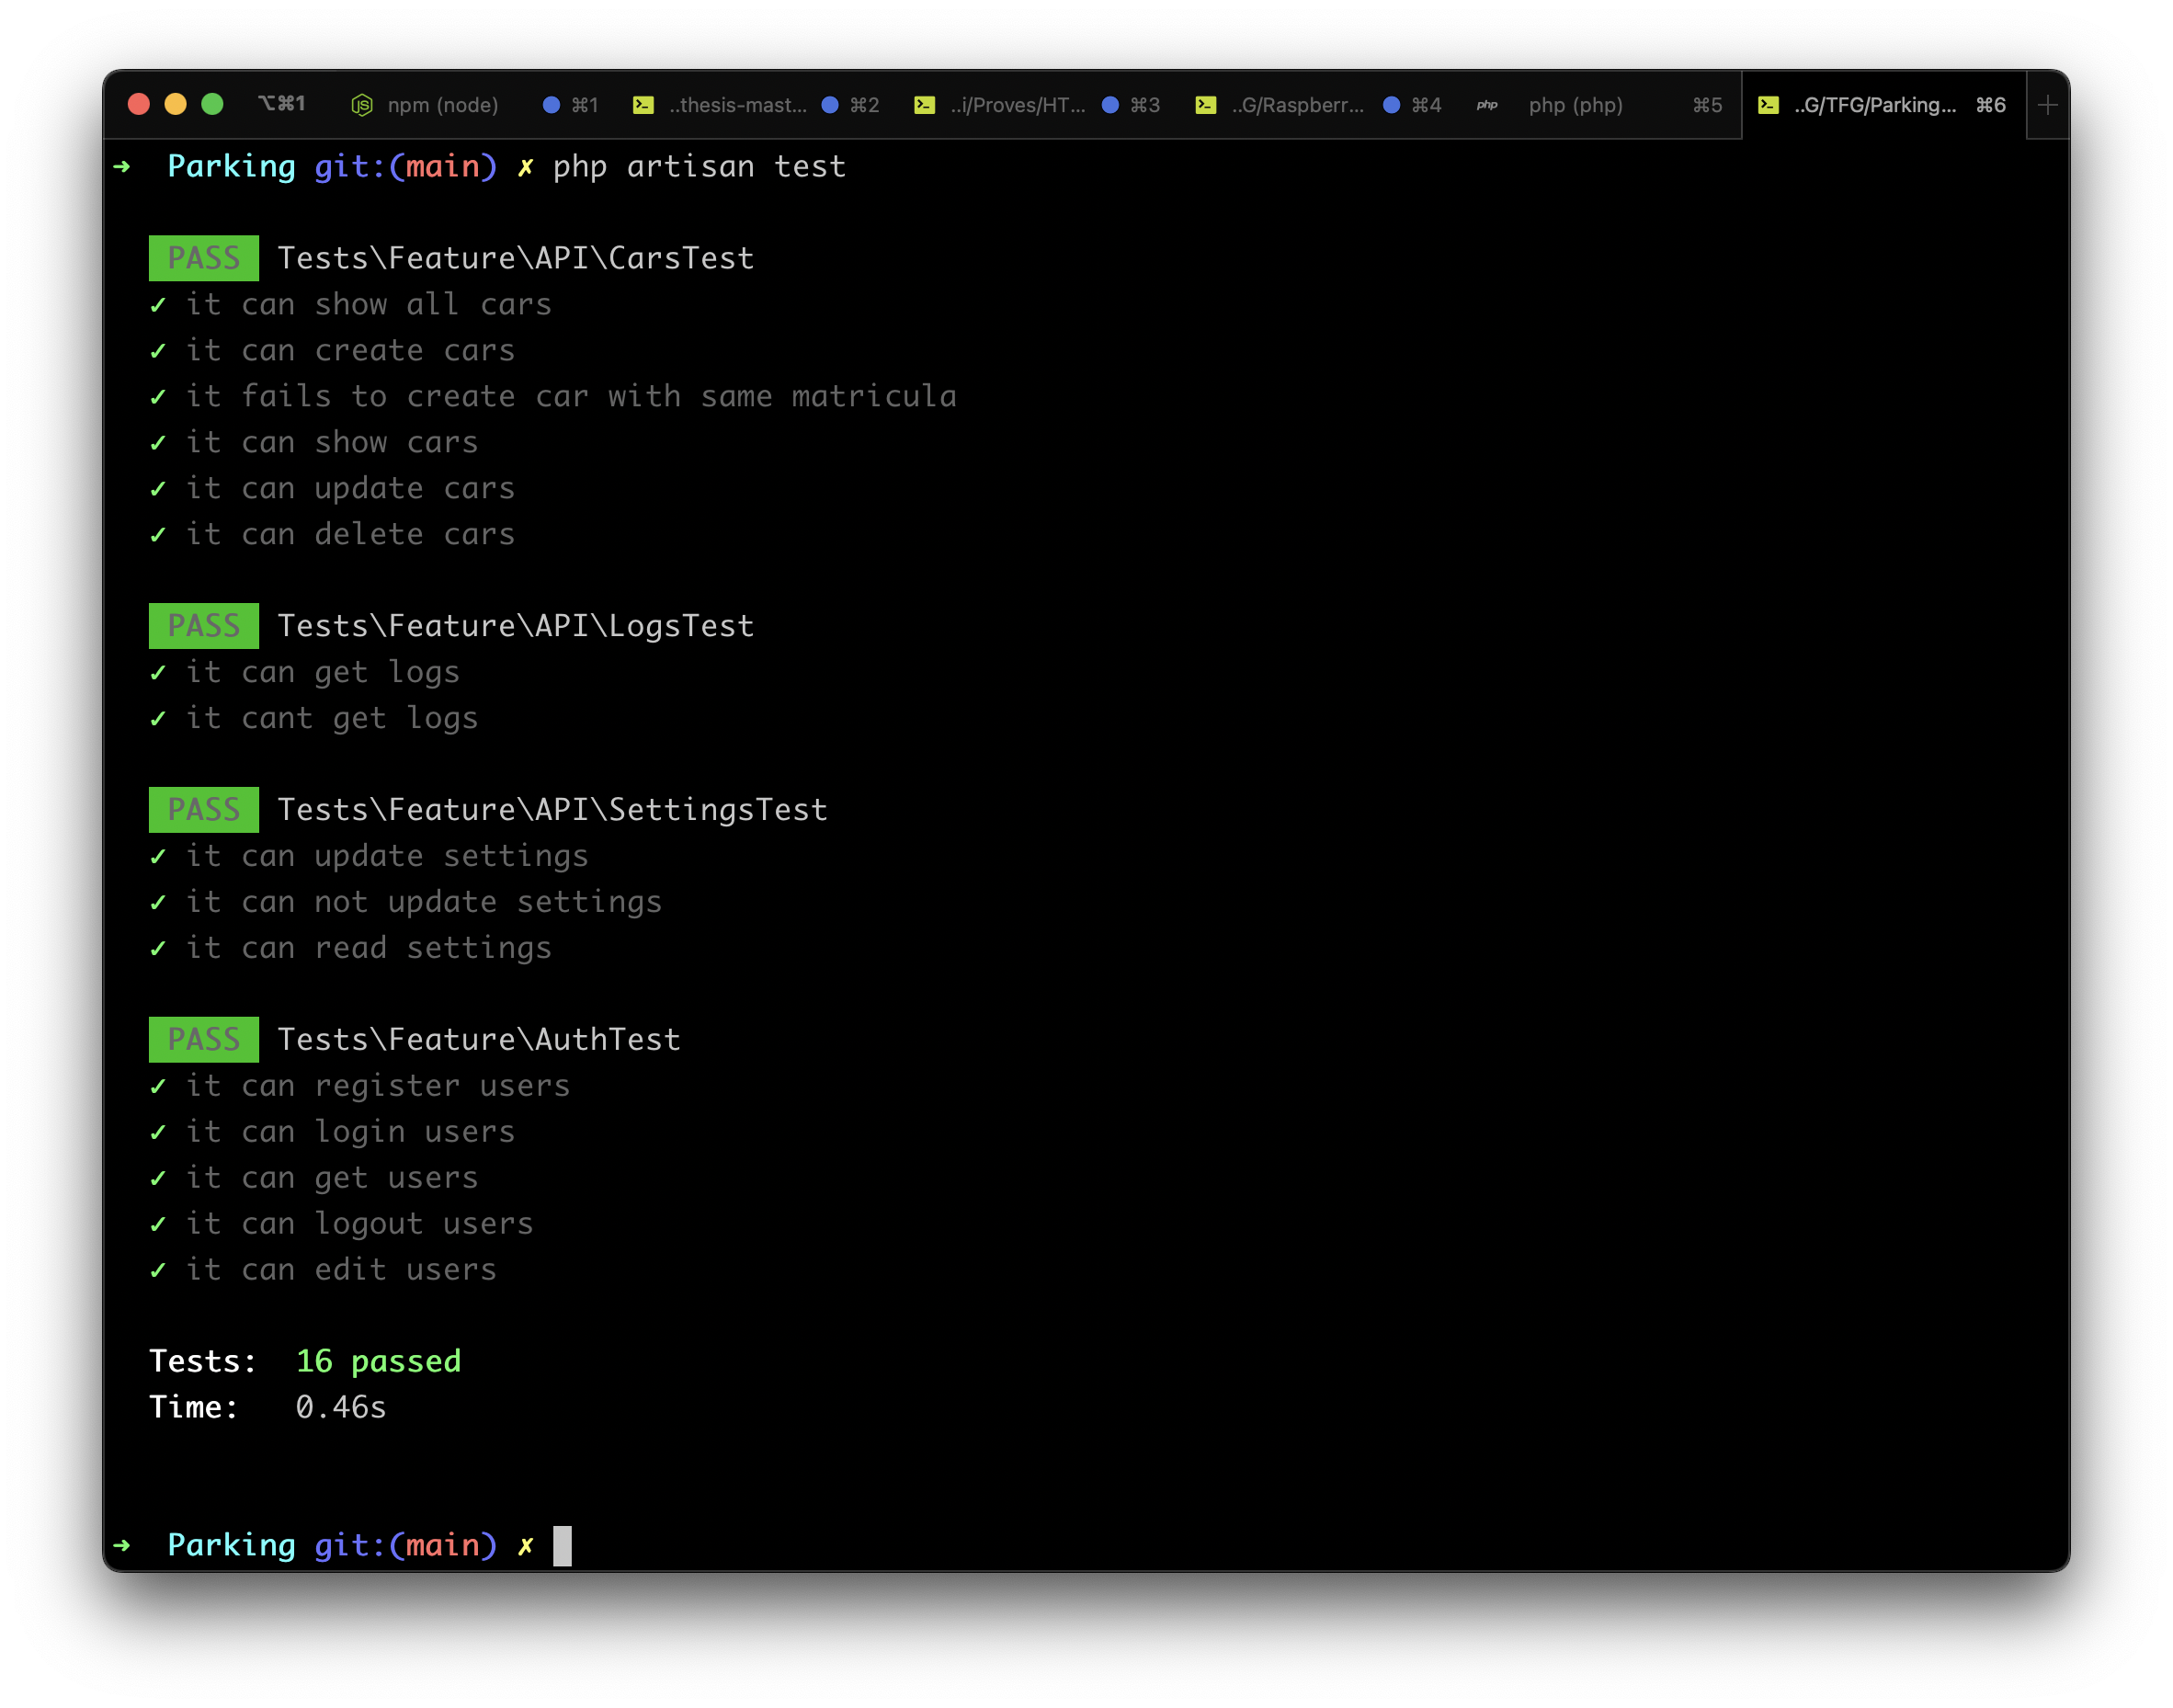
\includegraphics[scale=0.20]{Fotos/testsComprovacio.png}
    \end{center}
    \caption{Tests Correctes}
    \label{fig:register_photo}
\end{figure}